\documentclass{article}\usepackage{graphicx, color}
%% maxwidth is the original width if it is less than linewidth
%% otherwise use linewidth (to make sure the graphics do not exceed the margin)
\makeatletter
\def\maxwidth{ %
  \ifdim\Gin@nat@width>\linewidth
    \linewidth
  \else
    \Gin@nat@width
  \fi
}
\makeatother

\IfFileExists{upquote.sty}{\usepackage{upquote}}{}
\definecolor{fgcolor}{rgb}{0.2, 0.2, 0.2}
\newcommand{\hlnumber}[1]{\textcolor[rgb]{0,0,0}{#1}}%
\newcommand{\hlfunctioncall}[1]{\textcolor[rgb]{0.501960784313725,0,0.329411764705882}{\textbf{#1}}}%
\newcommand{\hlstring}[1]{\textcolor[rgb]{0.6,0.6,1}{#1}}%
\newcommand{\hlkeyword}[1]{\textcolor[rgb]{0,0,0}{\textbf{#1}}}%
\newcommand{\hlargument}[1]{\textcolor[rgb]{0.690196078431373,0.250980392156863,0.0196078431372549}{#1}}%
\newcommand{\hlcomment}[1]{\textcolor[rgb]{0.180392156862745,0.6,0.341176470588235}{#1}}%
\newcommand{\hlroxygencomment}[1]{\textcolor[rgb]{0.43921568627451,0.47843137254902,0.701960784313725}{#1}}%
\newcommand{\hlformalargs}[1]{\textcolor[rgb]{0.690196078431373,0.250980392156863,0.0196078431372549}{#1}}%
\newcommand{\hleqformalargs}[1]{\textcolor[rgb]{0.690196078431373,0.250980392156863,0.0196078431372549}{#1}}%
\newcommand{\hlassignement}[1]{\textcolor[rgb]{0,0,0}{\textbf{#1}}}%
\newcommand{\hlpackage}[1]{\textcolor[rgb]{0.588235294117647,0.709803921568627,0.145098039215686}{#1}}%
\newcommand{\hlslot}[1]{\textit{#1}}%
\newcommand{\hlsymbol}[1]{\textcolor[rgb]{0,0,0}{#1}}%
\newcommand{\hlprompt}[1]{\textcolor[rgb]{0.2,0.2,0.2}{#1}}%

\usepackage{framed}
\makeatletter
\newenvironment{kframe}{%
 \def\at@end@of@kframe{}%
 \ifinner\ifhmode%
  \def\at@end@of@kframe{\end{minipage}}%
  \begin{minipage}{\columnwidth}%
 \fi\fi%
 \def\FrameCommand##1{\hskip\@totalleftmargin \hskip-\fboxsep
 \colorbox{shadecolor}{##1}\hskip-\fboxsep
     % There is no \\@totalrightmargin, so:
     \hskip-\linewidth \hskip-\@totalleftmargin \hskip\columnwidth}%
 \MakeFramed {\advance\hsize-\width
   \@totalleftmargin\z@ \linewidth\hsize
   \@setminipage}}%
 {\par\unskip\endMakeFramed%
 \at@end@of@kframe}
\makeatother

\definecolor{shadecolor}{rgb}{.97, .97, .97}
\definecolor{messagecolor}{rgb}{0, 0, 0}
\definecolor{warningcolor}{rgb}{1, 0, 1}
\definecolor{errorcolor}{rgb}{1, 0, 0}
\newenvironment{knitrout}{}{} % an empty environment to be redefined in TeX

\usepackage{alltt}
\frenchspacing






\title{Biological shape as a weighted network}
\author{Peter D Smits \and Ben Frable}

\begin{document}
\maketitle


\section{Brief Introduction}
Here we envision biological shape, and the differences between shapes, as a network or graph model.
A network model is the depiction of the relationships between many nodes.
Each of these nodes may represent many different items or subjects of the same class.
In, for example, a social network is where each node represents a single person.
In this case, nodes represent a unique biological shape.

Between these nodes are links or edges.
In the social network example, an edge would represent a ``friendship'' or some other social connection between two individuals.
It is possible for edges to have weights, representing the degree of connectedness between two nodes.
Unlike in a distance matrix, a higher value represents a stronger connectedness.
Here, our edges represent the similarity of two shape configurations.
How these edges are assigned and weighted, however, is a via an extended procedure.

In network theory, a community is a densly connected set of nodes that are more connected to each other than to other groups.
In a given network, the number o groups may range between one large group and as many groups as there are nodes.
The shape network made from the matrix of \(\rho\) can then be analyzed using the various community detection algorithms in order to find if there are any subgroups of morphologies that are more densly connected.
These subgroups represent highly similar morphologies, and different communities/groups represent large scale differences in morphology.
Effectively, these community detection algorithms are defining different morphological categories directly from the morphological similarities as opposed to using prior knowledge or observation.


\section{Methodology}
The core of this entire process lies with the Riemannian shape distance, \(\rho\), between two configurations. 
A shape configuration is the set of landmarks that represent a unique shape. 
There are a technically infinite number of unique shapes, and our sample in geometric morphometric studies only represents a subset of the biologically known or possible shapes.

Shapes, when properly scaled and fit via some form of Procrustes analysis, exist not in a Euclidean plane, but on a Riemannian manifold.
Convenitnetly, a Riemannian manifold is metrizable and we can define some kind of metric to represent the ``distance'' between two shape configurations.
This Riemannian shape distance, \(\rho\) was defined by Kendall CITATION and varies between 0 and \(\pi /2\).
A value closer to 0 means that two shapes are closer in shape space, while a higher value indicates that two shapes are farther away in shape space.
Conveniently here is a function for calculating \(\rho\) in the {\tt{shapes}} package CITATION called {\tt{riemdist()}}.

The first step is the using generalized Procrustes analysis (GPA) to align all of our shapes and remove all non-shape elements.
After this a pairwise distance matrix is calculated for all shape combinations using {\tt{riemdist()}}. This produces a square \(n \cdot n\) matrix, where \(n\) is the number of unique shapes.
This pairwise \(\rho\) matrix represents how close every shape is to all other shapes.
From here, we want to determine which shapes are closer to each other than we would expect by random.
We require a Monte Carlo process to determine what ``random'' is.

How we define ``by random'' is very important here. Here, we are interested in a value of \(\rho\) smaller than than we would expect half of the time by random. This means, that we want to find which values of \(\rho\) are smaller than the median of a null distribution.


\subsection{Monte Carlo process}
The null distribution here is created from using two randomly selected shape configurations, moving the landmarks slightly to create two new, most likely valid, shape configuration.
\(\rho\) is then calculated for these two new shapes and stored.
This process is repeated many times in order to approximate a distribution of possible values of \(\rho\).
After determining this null distribution, all values greater than the median of this null distribution are removed.
The inverse of all remaining pairwise comparisons are then calculated, giving the future edge weights.
The resulting matrix is an undirected, weighted adjacency matrix which can easily be converted into a network for use in the {\tt{igraph}} package CITATION.

I've implemented this Monte Carlo process as a few functions in R.
The core function is {\tt{jitter.landmark()}}.
\begin{knitrout}\scriptsize
\definecolor{shadecolor}{rgb}{0.969, 0.969, 0.969}\color{fgcolor}\begin{kframe}
\begin{alltt}
jitter.landmark <- \hlfunctioncall{function}(land) \{
    \hlfunctioncall{for} (ii in \hlfunctioncall{seq}(\hlfunctioncall{ncol}(land))) \{
        land[, ii] <- land[, ii] + \hlfunctioncall{runif}(n = \hlfunctioncall{length}(land[, ii]), min = -(\hlfunctioncall{min}(\hlfunctioncall{abs}(\hlfunctioncall{diff}(land[, 
            ii])))), max = \hlfunctioncall{min}(\hlfunctioncall{abs}(\hlfunctioncall{diff}(land[, ii]))))
    \}
    land
\}
\end{alltt}
\end{kframe}
\end{knitrout}


This functions are called {\tt{nsim}} times (deafult 1000) by the {\tt{riem.distribution()}} function.
Using the original data set, {\tt{jitter.landmark()}} is called on {\tt{nsim}} two shape combinations.
A lambda function is used to calculate the reimanian distance for all of the {\tt{nsim}} combinations.
Currently, the lambda function executed as part of a call to {\tt{mclapply()}} which is a parallel function from the {\tt{parallel}} core package.
Currently, it will use the maximum number of cores avaliable and the seed is optimzed for reproducibility.
Without this feature, the process will run much slower.
This function will not work on non-POSIX systems (i.e. Windows).
\begin{knitrout}\scriptsize
\definecolor{shadecolor}{rgb}{0.969, 0.969, 0.969}\color{fgcolor}\begin{kframe}
\begin{alltt}
riem.distribution <- \hlfunctioncall{function}(fit.land, nsim = 1000) \{
    ran.land <- \hlfunctioncall{vector}(mode = \hlstring{"list"}, length = nsim)
    \hlfunctioncall{for} (ii in \hlfunctioncall{seq}(nsim)) \{
        s <- \hlfunctioncall{sample}(fit.land$n, 2)
        sh1 <- \hlfunctioncall{jitter.landmark}(fit.land$rotated[, , s[1]])
        sh2 <- \hlfunctioncall{jitter.landmark}(fit.land$rotated[, , s[2]])
        ran.land[[ii]] <- \hlfunctioncall{abind}(sh1, sh2, along = 3)
    \}
    res <- \hlfunctioncall{mclapply}(ran.land, \hlfunctioncall{function}(x) \{
        \hlfunctioncall{riemdis}(x[, , 1], x[, , 2])
    \}, mc.cores = \hlfunctioncall{detectCores}(), mc.set.seed = T)
    res
\}
\end{alltt}
\end{kframe}
\end{knitrout}


% All of the above functions can probably made much simpler.
% {\tt{jitter.landmark()}} can remain seperate while the entierty of {\tt{fit.riem()}} can be made a lambda function in the {\tt{mclapply()}} call in {\tt{riem.distribution()}}


The interface function {\tt{shape.simulation()}} outputs a quantile value necessary for determining our ``at random.'' The deafult quantile of 0.50 is the same as the median of a sample.
\begin{knitrout}\scriptsize
\definecolor{shadecolor}{rgb}{0.969, 0.969, 0.969}\color{fgcolor}\begin{kframe}
\begin{alltt}
shape.simulate <- \hlfunctioncall{function}(fit.land, nsim = 1000, probs = 0.5) \{
    ri.di <- \hlfunctioncall{riem.distribution}(fit.land, nsim = nsim)
    \hlfunctioncall{quantile}(\hlfunctioncall{unlist}(ri.di), probs = probs)
\}
\end{alltt}
\end{kframe}
\end{knitrout}


\subsection{Community detection}

There are currently eight different community detection algorithms implemented as part of the {\tt{igraph}} package.
Each of these algorithms try to optimze different communities based on various criteria.
For example, the ``walktrap'' algorithm determines communties by which sections of a graph a random walk is most frequently.
This algorithm, however, requires that there are no unconnected nodes, or nodes that have no edges.
Currently, I have tested the ``edge betweenness,'' ``fast-greedy,'' and ``leading eigenvector'' algorithms.
Each gives slightly different results, reflecting the method by which they determine couuminity presence and structure.

Implementation of these algorithms is illustrated below with gorilla and fish examples.
Additionally, I've included heirarchical clustering results from the pariwise \(\rho\) matrix for both of these examples.

\section{Examples}
\subsection{Gorilla vertebrae}
TODO

\subsection{Fish example}
The first step is to import the correct libraries and data files.
The functions described above are part of my script file, while the {\tt{readtps.R}} file is my fork of Ananda Mahto's original script GIST LINK.
This fork improves integration of .tps files and the {\tt{shapes}} package.
Additionally, becreporause this is a randomization process, for reproducibiliity it is necessary to manually set the seed value. Additionally, the RNG kind is changed to the L'Ecuyer algorithm CITATION which is the best for random number generationalgorithm implemented in R for parallel processes.
\begin{knitrout}\scriptsize
\definecolor{shadecolor}{rgb}{0.969, 0.969, 0.969}\color{fgcolor}\begin{kframe}
\begin{alltt}
\hlfunctioncall{require}(shapes)
\hlfunctioncall{require}(igraph)
\hlfunctioncall{require}(parallel)
\hlfunctioncall{require}(abind)
\hlfunctioncall{source}(\hlstring{"landmark_montecarlo.R"})
\hlfunctioncall{source}(\hlstring{"/home/peter/Documents/projects/3294254/readtps.R"})
\hlfunctioncall{RNGkind}(\hlstring{"L'Ecuyer-CMRG"})
\hlfunctioncall{set.seed}(1)
ano <- \hlfunctioncall{read.tps}(\hlstring{"AnostomidaeFinal.TPS"}, shapes = TRUE)
cur <- \hlfunctioncall{read.tps}(\hlstring{"CurimatidaeF.TPS"}, shapes = TRUE)
fish <- \hlfunctioncall{abind}(ano$landmark, cur$landmark)
\end{alltt}
\end{kframe}
\end{knitrout}


Next, we use GPA to fit our entire sample of 67 fish. We also calculate the pairwise \(\rho\) matrix. This is actually really dirty code that can probably be implemented as a single {\tt{outer}} call, but I've yet to figure it out.

\begin{knitrout}\scriptsize
\definecolor{shadecolor}{rgb}{0.969, 0.969, 0.969}\color{fgcolor}\begin{kframe}
\begin{alltt}
fish.fit <- \hlfunctioncall{procGPA}(fish)
riem.comp <- \hlfunctioncall{matrix}(0, ncol = fish.fit$n, nrow = fish.fit$n)
samp <- fish.fit$n
\hlfunctioncall{for} (ii in \hlfunctioncall{seq}(samp)) \hlfunctioncall{for} (kk in \hlfunctioncall{seq}(samp)) \{
    riem.comp[ii, kk] <- \hlfunctioncall{riemdist}(fish.fit$rotated[, , ii], fish.fit$rotated[, 
        , kk])
\}
\end{alltt}
\end{kframe}
\end{knitrout}


From this fit, we should examine our data to better understand what is going on initially. The basic ways are looking at the fitted landmarks (Figure \ref{fish-plotshapes}), the eigenscores from pricipal components analysis (Figure \ref{fish-pca}), and the thin-plate spine plot of an example fish to the mean shape (Figure \ref{fish-tps}.













\begin{figure}
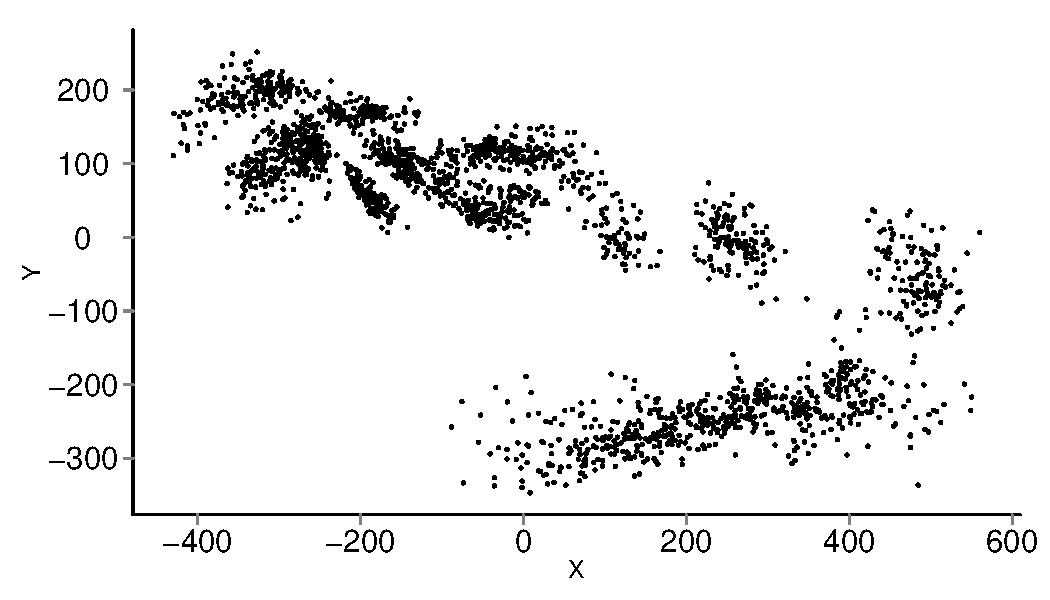
\includegraphics[height=0.3\textheight]{figure/fish-ex1}
\caption{Landmark positions of 66 of the fish taxa. One specimen is excluded.\label{fish-plotshapes}}
\end{figure}

\begin{figure}
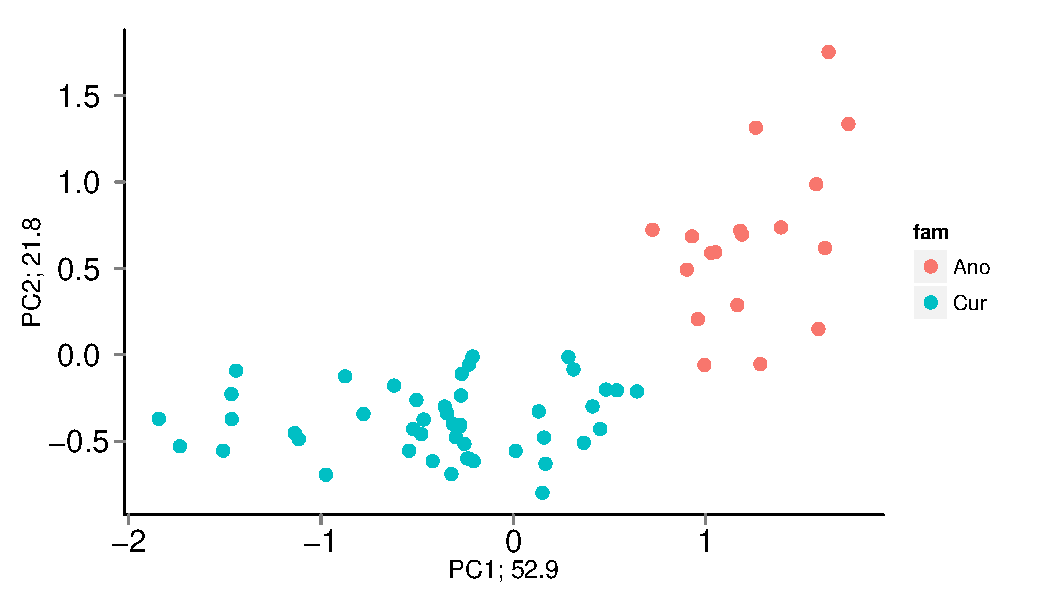
\includegraphics[height=0.3\textheight]{figure/fish-ex2}
\caption{PC1 versus PC2 for fish. Families are labeled. Percent of variation explained is included in axes labels. One specimen (42) is excluded.\label{fish-pca}}
\end{figure}

% \begin{figure}
% 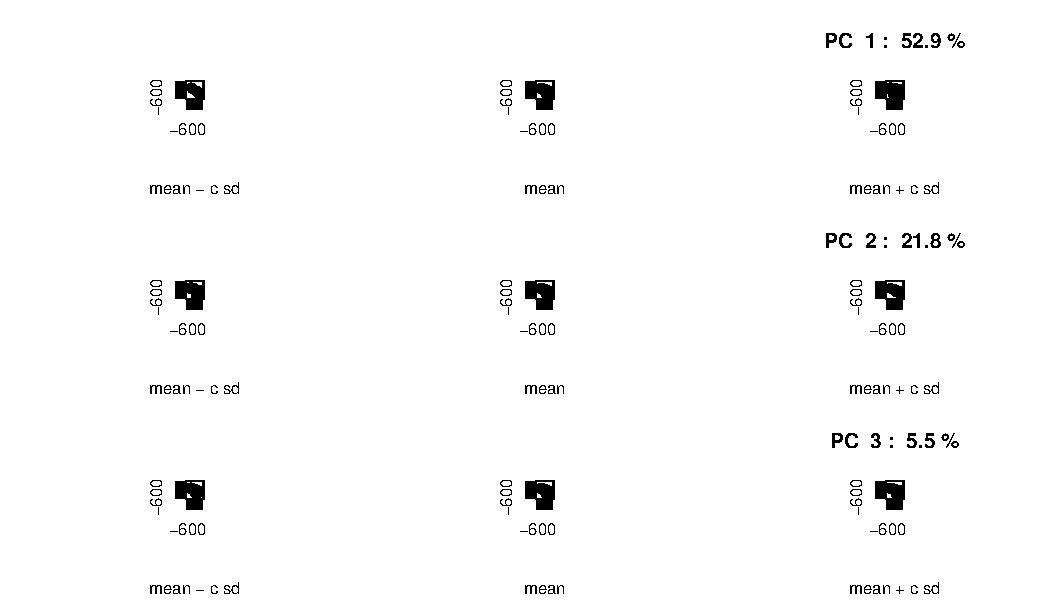
\includegraphics[width=\textwidth]{figure/fish-ex3}
% \caption{Alternative method for interpreting the principal components analysis.}
% \end{figure}

\begin{figure}
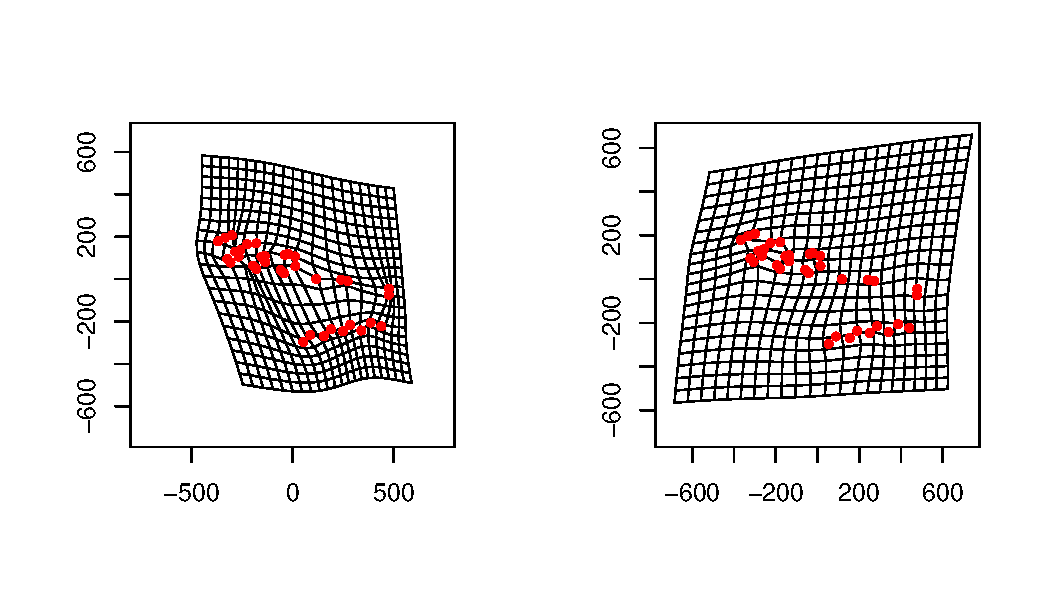
\includegraphics[height=0.35\textheight]{figure/fish-ex4}
\caption{TPS grids for Ano (right) and Cur (left).\label{fish-tps}}
\end{figure}

Following this, the Monte Carlo process is run so that we can begin to analyze the structure of our shape relationships.
This process is very long and takes many hours.
Those values which are greater than the median of the Monte Carlo distribution are discarted and the inverse of the remaining ones is calculated, producing a weighted adacency matrix.

\begin{knitrout}\scriptsize
\definecolor{shadecolor}{rgb}{0.969, 0.969, 0.969}\color{fgcolor}\begin{kframe}
\begin{alltt}
cutoff <- \hlfunctioncall{shape.simulate}(fish.fit, nsim = 10, probs = 0.5)
riem.comp[riem.comp > cutoff] <- 0
riem.comp[riem.comp != 0] <- 1/riem.comp[riem.comp != 0]
\end{alltt}
\end{kframe}
\end{knitrout}


The weighted adacency matrix is then transformed into a network and the three community detection algorithms are then used to analyze the resulting graph.

\begin{knitrout}\scriptsize
\definecolor{shadecolor}{rgb}{0.969, 0.969, 0.969}\color{fgcolor}\begin{kframe}
\begin{alltt}
data.graph <- \hlfunctioncall{graph.adjacency}(riem.comp, mode = \hlstring{"undirected"}, weighted = TRUE)
data.fc <- \hlfunctioncall{fastgreedy.community}(data.graph)
data.ebc <- \hlfunctioncall{edge.betweenness.community}(data.graph)
data.lec <- \hlfunctioncall{leading.eigenvector.community}(data.graph)
\end{alltt}
\end{kframe}
\end{knitrout}


We can then examine the results of these community detection algorithms. 
The simplest manner is the just view the graphic output.




In general, there are two identified communities.
These communities are not, however, identical to the two known families.
There is a group of ``Cur'' fish that are most morphologically similar to ``Ano'' fish.

The next step after this is determining if this graph is actually interesting.
This requires more reading.

\section{Concerns and Future Development}
\begin{enumerate}
\item I'm unsure how valid it is to define ``by random'' in the way that we did. 
I would need to actually talk to someone or read a lot to answer this one.

\item Need to make sure I'm not making invalid shape configurations

\item Unsure if I need to do {\tt{procGPA()}} every time in the MC process.

\item Choice of community detection algorithm.
This one just requires a lot of reading I think to figure out how exactly they differ. 

\item Are the edge weights to high?
Should they be rescaled

\item MC approach to understanding network.
{\tt{statnet}} packages.
Is the network different from random?

\item Model based clustering possibilities.
Can we classify without a network?
Would use the {\tt{mclust}} package CITATION, but there are awkward philosophical questions that come up with using that methodology.

\item Need to do some machine learning reading.
This project is essentially unsupervised clustering, but doing it in a weird way.

\end{enumerate}

\newpage
For reproducibility information.
\begin{knitrout}\scriptsize
\definecolor{shadecolor}{rgb}{0.969, 0.969, 0.969}\color{fgcolor}\begin{kframe}
\begin{alltt}
\hlfunctioncall{sessionInfo}()
\end{alltt}
\begin{verbatim}
## R version 2.15.1 (2012-06-22)
## Platform: x86_64-pc-linux-gnu (64-bit)
## 
## locale:
##  [1] LC_CTYPE=en_US.UTF-8       LC_NUMERIC=C              
##  [3] LC_TIME=en_AU.UTF-8        LC_COLLATE=en_US.UTF-8    
##  [5] LC_MONETARY=en_AU.UTF-8    LC_MESSAGES=en_US.UTF-8   
##  [7] LC_PAPER=C                 LC_NAME=C                 
##  [9] LC_ADDRESS=C               LC_TELEPHONE=C            
## [11] LC_MEASUREMENT=en_AU.UTF-8 LC_IDENTIFICATION=C       
## 
## attached base packages:
## [1] parallel  stats     graphics  grDevices utils     datasets  methods  
## [8] base     
## 
## other attached packages:
## [1] abind_1.4-0          igraph_0.6-2         shapes_1.1-5        
## [4] MASS_7.3-20          rgl_0.92.892         scatterplot3d_0.3-33
## [7] formatR_0.6          knitr_0.7           
## 
## loaded via a namespace (and not attached):
## [1] digest_0.5.2   evaluate_0.4.2 plyr_1.7.1     stringr_0.6.1 
## [5] tools_2.15.1  
\end{verbatim}
\end{kframe}
\end{knitrout}


\end{document}
